\chapter{IT Infrastructure Documentation and Incident Knowledge Management}

\section{Introduction}
This chapter forms the theoretical bridge between the study of existing solutions and the practical implementation of MapIT. Its purpose is to define the concepts that make the project meaningful: information systems, knowledge management, incident tracking, and relationship mapping. These ideas are not abstract decorations; they correspond directly to the structure that appears in the codebase and in the user interface.

\section{Information Systems as a Knowledge Infrastructure}
\subsection{Definition of an information system}
An information system is an organized combination of people, processes, data, and technology that transforms raw data into usable information and supports operational decision-making \cite{laudon_mis,pressman}. In MapIT, this definition appears in the separation between the React/Next.js user interface, the Express backend API, the PostgreSQL database, and the permission middleware. The result is not just a website, but a small knowledge infrastructure for IT operations.

\subsection{Definition of IT documentation}
IT documentation can be defined as the structured and continuously maintained set of records that describes infrastructure components, operating procedures, dependencies, incidents, and decisions. Its role is to preserve operational memory so that technical teams can understand what exists, how it behaves, and what was done previously to maintain or restore it. In an IT service context, documentation is only useful when it is accurate, searchable, and tied to the real workflow of the organization \cite{itil4,km}.

Table~\ref{tab:it-doc-impact} summarizes the operational effect of documentation quality on daily IT work.

\begin{table}[H]
\centering
\small
\renewcommand{\arraystretch}{1.15}
\begin{tabular}{|p{0.30\textwidth}|p{0.30\textwidth}|p{0.30\textwidth}|}
\hline
\textbf{Feature} & \textbf{With Documentation} & \textbf{Without Documentation} \\ \hline
\textbf{Troubleshooting} & Fast, efficient & Slow, error-prone \\ \hline
\textbf{Onboarding} & Clear, structured & Confusing, inconsistent \\ \hline
\textbf{Compliance} & Easier to prove & Risk of violations \\ \hline
\textbf{Knowledge Sharing} & Smooth & Dependent on individuals \\ \hline
\textbf{System Reliability} & Higher & Lower \\ \hline
\end{tabular}
\caption{Impact of documentation on IT operations}
\label{tab:it-doc-impact}
\end{table}

\subsection{From data to operational knowledge}
MapIT stores data such as asset names, incident titles, problem descriptions, relationship types, and audit entries. That data becomes information when it is organized into pages, filters, status flows, or summary reports. It becomes operational knowledge when a technician can reuse it to answer a new incident, understand a dependency, or validate a corrective action. This progression is exactly why the application includes incidents, problems, documents, search, and feedback on knowledge suggestions.

Figure~\ref{fig:data-to-knowledge-chain} summarizes this progression in a simple visual chain.

\begin{figure}[H]
\centering
\fbox{\parbox{2.8cm}{\centering Raw data}}
\hspace{0.25cm}$\rightarrow$\hspace{0.25cm}
\fbox{\parbox{3.4cm}{\centering Structured information}}
\hspace{0.25cm}$\rightarrow$\hspace{0.25cm}
\fbox{\parbox{3.3cm}{\centering Operational knowledge}}
\hspace{0.25cm}$\rightarrow$\hspace{0.25cm}
\fbox{\parbox{2.8cm}{\centering Reuse and action}}
\caption{From data to reusable knowledge}
\label{fig:data-to-knowledge-chain}
\end{figure}

\subsection{Why the concept matters for MapIT}
The application is designed to preserve the technical memory of the infrastructure. A dashboard, a relationship graph, a search index, and a report summary all help the user see the system as a whole. In theoretical terms, MapIT is an information system that supports knowledge capture and knowledge retrieval in the same operational flow.

\section{Knowledge Management in IT Operations}
\subsection{Knowledge capture and reuse}
Knowledge management is the discipline of capturing experience, organizing it, validating it, and making it reusable \cite{davenport_prusak,nonaka_konno,km}. In MapIT, the reusable layer appears in problems with solutions, incidents with suggested knowledge, and documents that can be consulted later. The \texttt{IncidentKnowledgeFeedback} entity makes this process explicit by letting users state whether a suggested item was helpful.

\subsection{Knowledge quality and traceability}
Operational knowledge must be reliable, not merely available. That is why MapIT keeps audit logs, permission checks, and user-specific settings. The platform must know who changed a record, when it was changed, and under which permission level the action was executed. Without that traceability, the knowledge base would lose credibility in a real operational context.

\subsection{Why this is important for IT teams}
In an IT support environment, a good answer is not enough unless it can be found quickly and trusted. MapIT addresses this by indexing assets, problems, incidents, and documents through global search, by separating read access from management actions, and by exposing the operational state through a dashboard and reports. This is knowledge management as an operational practice, not just a repository.

\section{Incident Tracking and Relationship Mapping}
\subsection{Incident tracking}
Incident tracking is the formal recording of an incident from its opening to its closure, aligned with service management principles \cite{itil4,iso20000,atlassian_incident}. In the backend, MapIT uses a controlled incident lifecycle with the statuses \texttt{OPEN}, \texttt{IN\_PROGRESS}, \texttt{BLOCKED}, \texttt{RESOLVED}, and \texttt{CLOSED}. The detail page also supports priority, assignment, team ownership, and changes to status. This matters because it reflects the lifecycle discipline expected in modern service operations.

Figure~\ref{fig:incident-flow} illustrates the knowledge-reuse loop that follows an incident.

\begin{figure}[H]
\centering
	\fbox{\parbox{2.9cm}{\centering Incident record}}
	\hspace{0.2cm}$\rightarrow$\hspace{0.2cm}
	\fbox{\parbox{3.2cm}{\centering Root cause analysis}}
	\hspace{0.2cm}$\rightarrow$\hspace{0.2cm}
	\fbox{\parbox{3.0cm}{\centering Knowledge article}}
	\hspace{0.2cm}$\rightarrow$\hspace{0.2cm}
	\fbox{\parbox{2.8cm}{\centering Search and reuse}}
	\caption{Knowledge reuse cycle in IT operations}
\label{fig:incident-flow}
\end{figure}

\subsection{Relationship mapping}
Relationship mapping is the representation of dependency between infrastructure elements. In MapIT, relationships are stored as directed links between assets and visualized in a graph where the user can drag nodes, zoom, filter asset types, and inspect the connections. This feature is not decorative: it allows the user to reason about impact, identify upstream and downstream dependencies, and understand which asset relationships are affected by a failure.

\subsection{Why both concepts are essential}
Incident tracking gives the temporal view of a problem; relationship mapping gives the structural view of the infrastructure. Modern IT environments need both because a single incident can affect multiple assets, and a single asset can be implicated in multiple incidents over time. MapIT combines these two views so that the user can move from a symptom to a dependency to a reusable solution.

\section{Applying the Theory to MapIT}
\subsection{The MapIT domain model}
The Prisma schema shows how the theoretical concepts become concrete entities: \texttt{User}, \texttt{Incident}, \texttt{Document}, \texttt{Asset}, \texttt{Problem}, \texttt{Relationship}, \texttt{Role}, \texttt{Permission}, \texttt{AuditLog}, \texttt{UserSettings}, and \texttt{IncidentKnowledgeFeedback}. These objects reflect the real domain of the project and show that MapIT is centered on operational knowledge rather than on general content management.

Figure~\ref{fig:mapit-class-diagram} gives a schema view of these entities and their relationships.

\begin{figure}[H]
\centering
	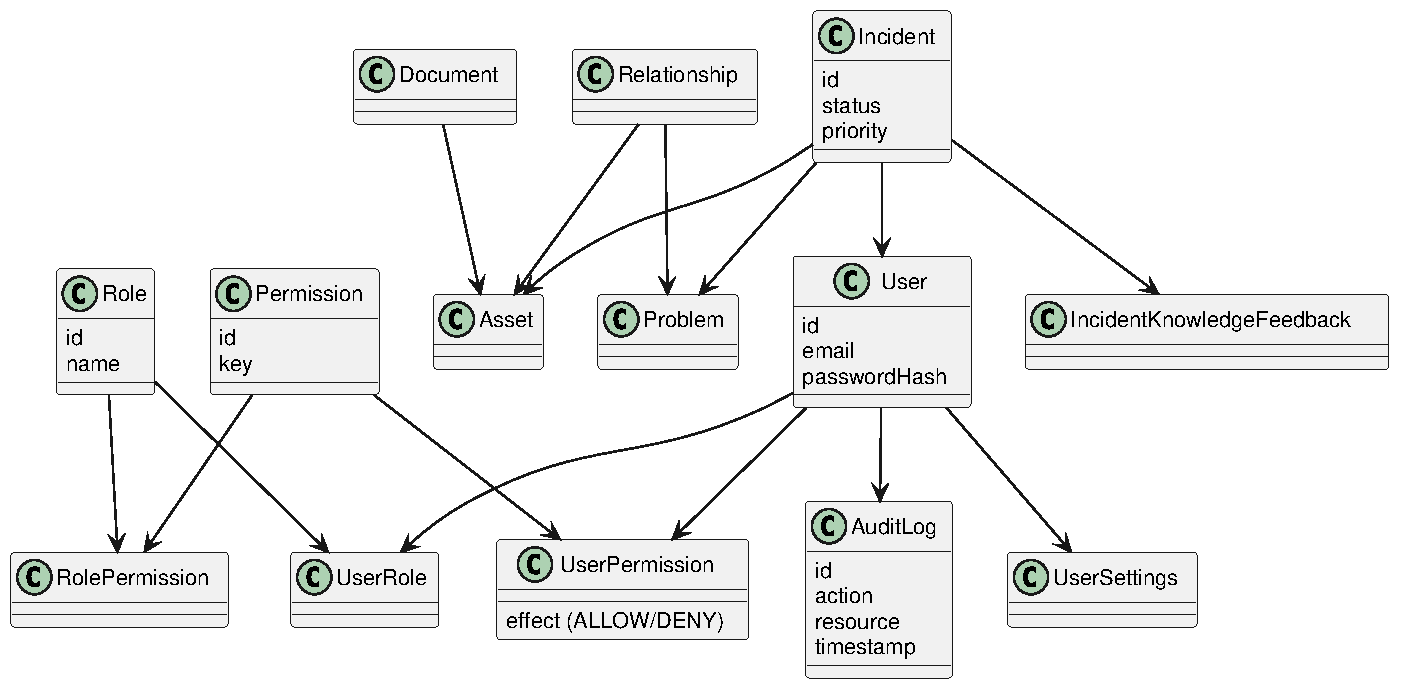
\includegraphics[width=0.95\textwidth]{figures/diagrams/simplified_class_diagram.pdf}
\caption{MapIT domain class diagram}
\label{fig:mapit-class-diagram}
\end{figure}

\subsection{How the theory appears in the interface}
The theory is visible in the frontend as well. The login page controls entry, the dashboard summarizes the environment, the incident detail page supports lifecycle actions, the asset pages show related problems and relationships, the search page unifies access to all knowledge, and the settings page exposes access control and audit logs. The access-control logic also follows common RBAC terminology used in enterprise systems \cite{microsoft_rbac}. This is the practical embodiment of the theoretical concepts defined in the chapter.

\subsection{Consistency of the theoretical path}
The theoretical path of this chapter moves from the definition of the domain to analysis, modeling, and realization. MapIT follows this logic through a practical IT infrastructure knowledge-management use case. The academic rigor is preserved by defining the concepts, justifying the approach, and showing how the implementation proves the model.

\section{Chapter Conclusion}
MapIT is grounded in established notions of information systems and knowledge management, but it applies them to a very specific IT operations problem: keeping infrastructure knowledge centralized, visual, and actionable. Incident tracking and relationship mapping are therefore core academic concepts for the project, not side features. The next chapter will show how these concepts were translated into the concrete software architecture and user-facing pages.
